% Newtonian Taylor--Culick retraction at arbitrary Ohnesorge number.
% Companion to validation-viscous (Trouton/Ahsan) and validation-inertial
% (FEM versus Basilisk at Oh_SB < 0.1).
%
% Build: see README.md
\documentclass[11pt,a4paper]{article}

\usepackage[margin=2.4cm]{geometry}
\usepackage{amsmath,amssymb}
\usepackage{graphicx}
\usepackage{booktabs}
\usepackage[hidelinks]{hyperref}
\usepackage{caption}

\newcommand{\Ohsb}{\mathrm{Oh}_{\mathrm{SB}}}
\newcommand{\Ohp}{\mathrm{Oh}_{p}}
\newcommand{\Vtc}{V_{TC}}
\newcommand{\ustar}{u^{*}}
\newcommand{\tstar}{t^{*}}

\title{Newtonian Taylor--Culick retraction at arbitrary Ohnesorge number}
\author{%
  Vatsal Sanjay\thanks{%
    \href{mailto:vatsal.sanjay@comphy-lab.org}{vatsal.sanjay@comphy-lab.org};
    ORCID \href{https://orcid.org/0000-0002-4293-6099}{0000-0002-4293-6099}.}\\[2pt]
  \normalsize CoMPhy Lab, Department of Physics, Durham University,\\
  \normalsize Science Laboratories, South Road, Durham DH1 3LE, United Kingdom}
\date{\today}

\begin{document}
\maketitle

\begin{abstract}
A freely suspended planar liquid sheet, initially at rest, retracts under its
own surface tension. The collected mass gathers in a growing rim. Taylor
\cite{taylor1959} and Culick \cite{culick1960} predicted a terminal speed
$\Vtc = \sqrt{2\sigma/(\rho h_0)}$ from a global momentum budget, independent
of viscosity. Appendix~A of Sanjay \textit{et al.}\ \cite{sanjay2022} treated
the Newtonian problem at a single film Ohnesorge number with a two-phase
volume-of-fluid method. Here we sweep Ohnesorge number with a single-phase
sharp-interface finite-element method in a frame co-moving with the rim.
The recovered tip speed approaches $\Vtc$ at every $\Ohsb$ in the production
range $0.035$ to $1$. In a middle band $0.14724 \le \Ohsb \le 1$ the deficit
follows
$1 - \ustar = (1/(2\sqrt{\pi}))\,\sqrt{\Ohsb/\tstar}$
to within $1\%$. That coefficient is not universal on the evidence available.
It departs at both ends of the Ohnesorge range. The strongly inertial end,
$\Ohsb < 0.1$, is closed against $\Vtc$ and against an independent Basilisk
calculation rather than against lubrication curves. The one-dimensional
long-wave model and the two-dimensional Navier--Stokes solution cannot agree
across $\mathrm{Oh}$ in principle, because their deficits decay as
$(t^{*})^{-2}$ and $(t^{*})^{-1/2}$ respectively.
\end{abstract}

\section{Problem}
\label{sec:problem}

A semi-infinite planar liquid sheet of uniform thickness $h_0$, initially at
rest, retracts under its own surface tension $\sigma$. Surface tension pulls
the free edge back. The collected mass accumulates in a growing rim. There is
no surrounding gas. The interface is a true free surface with a stress
condition on it, not an interface between two resolved fluids.

Taylor \cite{taylor1959} and Culick \cite{culick1960} obtained the terminal
retraction velocity by balancing the capillary pull against the rate of
momentum gain of the rim,
\begin{equation}
  2\sigma = \rho h_0 \Vtc^{2}
  \qquad\Rightarrow\qquad
  \Vtc = \sqrt{2\sigma/(\rho h_0)}.
\end{equation}
The velocity is set by a global momentum budget, so it is independent of
viscosity. Viscosity controls only how the sheet approaches $\Vtc$, and how
long it takes.

Figure~\ref{fig:schematic} shows the computational setup. This note is intended
as an extension of Appendix~A of Sanjay \textit{et al.}\ \cite{sanjay2022},
which treated the classical retraction at a single film Ohnesorge number
($\mathrm{Oh}_f = 0.05$) with Basilisk \cite{basilisk}. The numerical method
here is different in kind. A single-phase, sharp-interface finite-element
method in a frame co-moving with the rim, built on pyoomph \cite{diddens2023}
and oomph-lib \cite{heil2006}. The inertial planar comparison against Basilisk
at $\Ohsb < 0.1$ is closed and is reported in the companion inertial note. The
one-dimensional Trouton/Ahsan work is the viscous-limit note.

\begin{figure}[htbp]
  \centering
  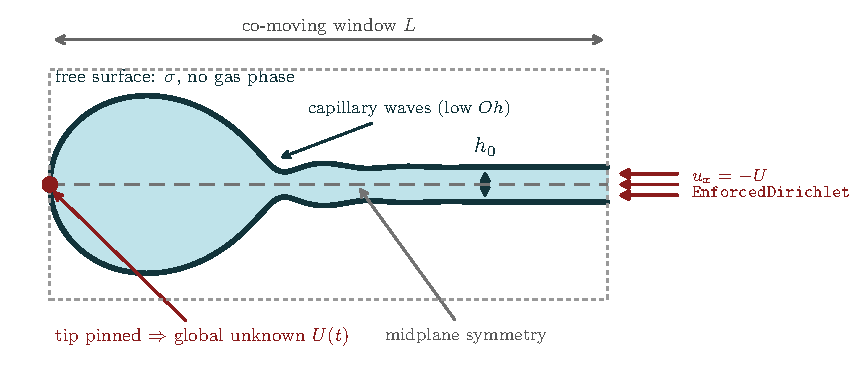
\includegraphics[width=\textwidth]{figures/fig1_schematic.pdf}
  \caption{Planar sheet of thickness $h_0$ retracting to the left. The
  computation is performed in a frame co-moving with the rim. The tip is pinned
  at the origin and the frame velocity $U(t)$ is promoted to a global unknown.
  The far field enters at $-U$ through a Lagrange-multiplier condition. Only
  the upper half is solved. The midplane is a symmetry line. At low
  $\mathrm{Oh}$ a train of decaying capillary waves runs ahead of the rim. The
  sheet outline is a computed interface, $\Ohsb = 0.035$ at $t \approx 15$.}
  \label{fig:schematic}
\end{figure}

\section{Non-dimensionalisation}
\label{sec:units}

Three conventions appear in this literature and they do not agree. Getting this
wrong moves the answer by exactly $\sqrt{2}$, which is large enough to look
like physics.

This code scales on the full thickness $h_0$, the density $\rho$ and the
surface tension $\sigma$, so that $\rho = \sigma = h_0 = 1$ and the
half-thickness is $0.5$.

\begin{center}
\begin{tabular}{ll}
\toprule
quantity & scale \\
\midrule
length & $h_0$ \\
velocity & $\sqrt{\sigma/(\rho h_0)}$ \\
time & $\sqrt{\rho h_0^{3}/\sigma}$ \\
Ohnesorge & $\mathrm{Oh} = \mu/\sqrt{\rho\sigma h_0}$ \\
\bottomrule
\end{tabular}
\end{center}

Sanjay \textit{et al.}\ \cite{sanjay2022} scale velocity on $\Vtc$ itself.
Savva \& Bush \cite{savva2009} use the same velocity scale and the same
Ohnesorge definition as that paper, but a viscous clock
$\tau_{\mathrm{vis}} = \mu H/(2\gamma)$ with $H$ the full thickness, so
$H \equiv h_0$. Sanjay \textit{et al.}\ and Savva \& Bush therefore share an
identical Ohnesorge convention. This code differs from both by $\sqrt{2}$,
\begin{equation}
  \Ohsb = \mathrm{Oh}_f = \mathrm{Oh}_{\mathrm{code}}/\sqrt{2}.
\end{equation}
The coded $\mathrm{Oh} = 0.05$ used to match the Basilisk study is
$\Ohsb = 0.035$. In code units, $\tau_{\mathrm{vis}} = \mu/2$. Throughout this
document $\mathrm{Oh}$ means $\Ohsb$, because that is what the published
comparison curves use. The velocity is reported as $\ustar = U/\Vtc$, which is
directly comparable across all three conventions and tends to $1$.

\section{Numerical framework}
\label{sec:method}

Incompressible Navier--Stokes is solved in the liquid only,
\begin{equation}
  \rho\bigl(\partial_t\mathbf{v} + \mathbf{v}\cdot\nabla\mathbf{v}\bigr)
  = -\nabla p + \nabla\cdot(2\mu\boldsymbol{\mathcal{D}}),
  \qquad
  \nabla\cdot\mathbf{v} = 0,
\end{equation}
with the free surface carrying the stress condition
$(-p I + 2\mu\boldsymbol{\mathcal{D}})\cdot\mathbf{n} = \sigma\kappa\mathbf{n}$.
There is no gas phase, hence no density ratio, no viscosity ratio, no diffuse
interface and no spurious-current budget to defend. That is the principal
methodological difference from the Basilisk study, which resolves both phases
with a volume-of-fluid tracer and a Brackbill surface-tension force.

The retraction path is long. The tip travels $\sim\Vtc\, t$, so a
laboratory-frame domain must contain the entire excursion. The Basilisk study
handled that with a domain $100\,h_0$ wide. Here the rim velocity is promoted
to a single global degree of freedom $U(t)$, fixed by a Lagrange multiplier
that pins the tip at the origin. The far field enters at $-U$. The mesh then
only has to cover a window around the rim, and $U(t)$ is itself the physical
observable.

The window must contain the viscous footprint $\sqrt{4\nu t}$, which grows with
$\mu$, so the required window grows with $\mathrm{Oh}$. The campaign is bounded
at $\Ohsb \le 1$. Beyond that the cost grows sharply for the strongly viscous
limit where no rim forms and the curves collapse. $\Ohsb \sim 1$ is where
inertia and viscosity are comparable.

The solver uses BDF2 with adaptive time stepping. The output cadence sets the
timestep, because $\mathrm{maxstep}$ is clamped to the current output interval
and the temporal-error estimator never binds. The number of output points is
therefore a physics-relevant parameter, exposed as \texttt{--n-outputs}.
Section~\ref{sec:timestep} shows that the campaign values are not sensitive to
it at any level that matters.

\section{Phenomenology}
\label{sec:pheno}

\begin{figure}[htbp]
  \centering
  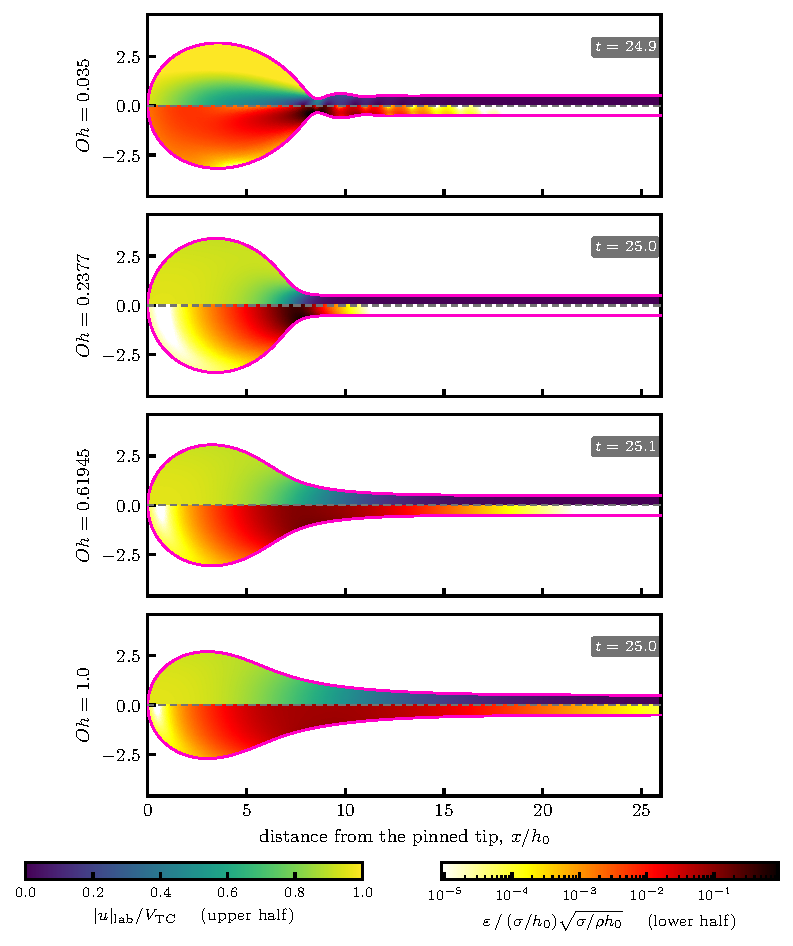
\includegraphics[width=\textwidth]{figures/fig2_phenomenology.pdf}
  \caption{Velocity magnitude (upper half) and viscous dissipation rate
  $\varepsilon = 2\mu\,\boldsymbol{\mathcal{D}}:\boldsymbol{\mathcal{D}}$ (lower half) at a
  common inertio-capillary time $t \approx 25$, over a factor-$29$ range in
  $\mathrm{Oh}$. Distances are from the pinned tip in units of $h_0$. Velocity
  is in the laboratory frame, so the undisturbed film reads zero. Colour scales
  are shared across the panels.}
  \label{fig:phenomenology}
\end{figure}

Figure~\ref{fig:phenomenology} is the sequence. At $\Ohsb = 0.035$ a nearly
circular rim is connected to the film by a distinct neck, with a train of
decaying capillary waves running ahead of it, as Savva \& Bush \cite{savva2009}
and Brenner \& Gueyffier \cite{brenner1999} describe for $\mathrm{Oh} < 0.1$.
At $\Ohsb = 0.2377$ the rim is still compact but the waves have gone. At
$\Ohsb = 0.61945$ the neck has washed out. At $\Ohsb = 1$ there is no distinct
rim. The sheet thickens over a broad region. The rim height at fixed $t$ is
remarkably insensitive to $\mathrm{Oh}$, because the mass collected is set by
the retraction velocity, which is itself $\mathrm{Oh}$-independent. What
changes is how that mass is distributed.

\begin{figure}[htbp]
  \centering
  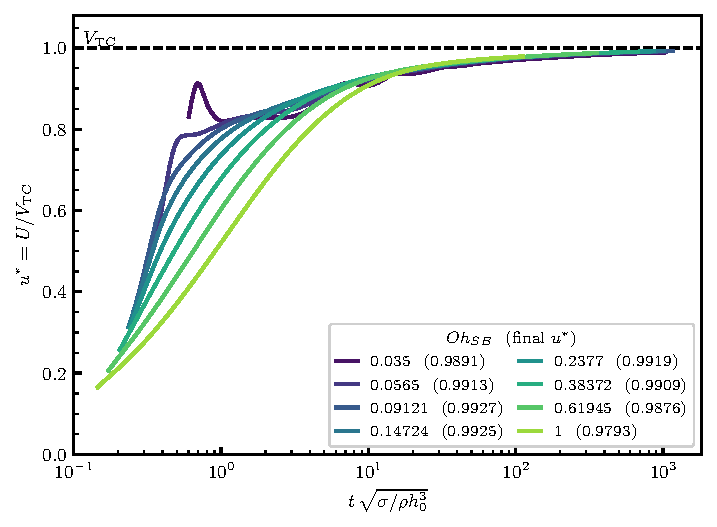
\includegraphics[width=\textwidth]{figures/fig3_velocity.pdf}
  \caption{Recovered control velocity $\ustar = U/\Vtc$ against the
  inertio-capillary clock for the eight-point sweep, $\Ohsb = 0.035$ to $1$.
  The time axis is logarithmic because the solver writes on a geometric output
  schedule. Two features are physical. The low-$\mathrm{Oh}$ overshoot near
  $t \approx 0.7$, where the rim first forms, and the late-time ripples at
  $\mathrm{Oh} \le 0.1$, which are the capillary-wave train beating against the
  rim.}
  \label{fig:velocity}
\end{figure}

\begin{figure}[htbp]
  \centering
  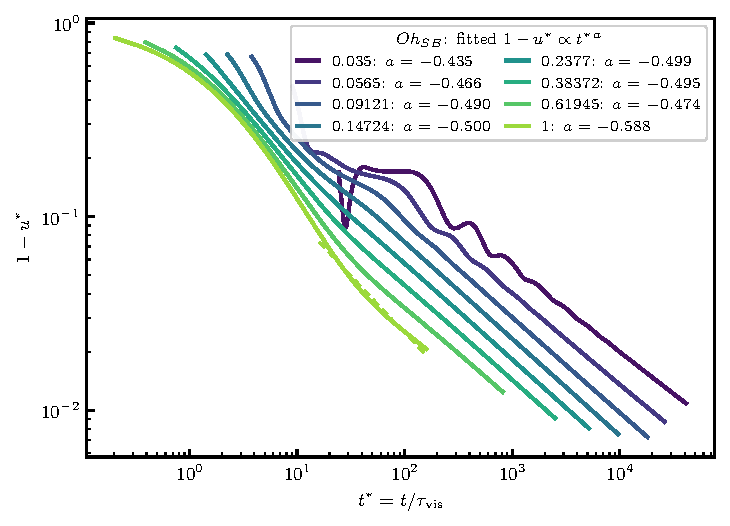
\includegraphics[width=\textwidth]{figures/fig4_approach.pdf}
  \caption{The same data as the gap $1 - \ustar$ against the viscous clock
  $\tstar = t/\tau_{\mathrm{vis}}$, on log--log axes. Dashed lines are
  least-squares fits over the last decade of each record.}
  \label{fig:approach}
\end{figure}

Figure~\ref{fig:velocity} is the observable the campaign exists to measure.
Every case is still climbing at the end of its production record. None reached
the $\ustar = 0.995$ target the sweep was sized for. The long inertial runs
later closed that approach against $\Vtc$ itself. Figure~\ref{fig:approach}
shows why a single global fit of the deficit is not usable if the record is
short. The exponent in $1 - \ustar \propto (t^{*})^{a}$ runs from $-0.435$ at
$\Ohsb = 0.035$ to $-0.588$ at $\Ohsb = 1$ on those production windows. Longer
records, reported in \S\ref{sec:established}, put the middle of the sweep on
$-1/2$.

\section{The one-dimensional reduced model}
\label{sec:oned}

Savva \& Bush's analysis is a long-wave (Trouton) reduction of the same
problem \cite{trouton1906,savva2009}. An independent finite-element
implementation of that model lives in the repository so that a disagreement
with their published figures can be attributed to digitisation, model, or
code. It reproduces the early-time asymptote $\ustar \to \sqrt{\tstar/\pi}$
and the exact tip growth $h = 1 + t/(2\mu)$. Richardson extrapolation at
$\Ohsb = 1$ gives $\ustar(30) \to 0.98073$ as $\mathrm{d}t \to 0$. Against
$0.95026$ from the two-dimensional finite-element method and $0.9542$ from the
digitised Savva \& Bush curve, the converged one-dimensional value is $3.2\%$
and $2.8\%$ high. An earlier report of a clean three-way agreement was an
artefact of an under-resolved timestep.

The bulk capillary term is switched off in that solver. Savva \& Bush's tip
closure already is the capillary pull of the massless cap, so a bulk curvature
term double-counts it. That is a physical argument supported by agreement, not
a derivation. The detailed Trouton/Ahsan campaign, including an independent
transcription of the code released with Ahsan \textit{et al.}\
\cite{ahsan2025}, is the viscous-limit note.

\section{Verification}
\label{sec:verify}

\subsection{Window, not mesh}

At $\Ohsb = 1$, $\tstar = 30$, mesh resolution $0.03/0.04/0.06$ and temporal
tolerance agree to better than $0.01\%$. At window length $L = 12$ that
agreement is around $\ustar = 0.8191$, which is domain-limited.

\begin{center}
\begin{tabular}{lr}
\toprule
$L$ & $\ustar(\tstar = 30)$ \\
\midrule
$12$ & $0.81910$--$0.81915$ \\
$16$ & $0.91443$ \\
$25$ & $0.94942$ \\
$40$ & $0.95026$ \\
$60$ & $0.95026$ \\
\bottomrule
\end{tabular}
\end{center}

The window length, not the mesh, is the controlling parameter, and it is
converged for $L \ge 40$. A well-converged mesh on too small a window is the
single easiest way to get a confidently wrong answer on this problem.

\subsection{Savva \& Bush}
\label{sec:savva}

Converged $\ustar(\tstar = 30) = 0.95026$ at $\Ohsb = 1$ sits $0.41\%$ below
the digitised Savva \& Bush figure-6 value of $0.9542$. At $\Ohsb = 0.5$ the
code gives $0.9297$ against their $\approx 0.93$. The $0.41\%$ offset is not a
timestep, mesh, or domain artefact. Whether it is digitisation error, a
long-wave modelling error, or a genuine difference between the lubrication
model and Navier--Stokes is the question flagged in \S\ref{sec:oned}.

\subsection{Timestep}
\label{sec:timestep}

Because $\mathrm{d}t$ is set by the output cadence, the campaign values were
checked against it at $\Ohsb = 1$, $\tstar = 30$, $L = 40$.

\begin{center}
\begin{tabular}{lrr}
\toprule
\texttt{n-outputs} & $\ustar(30)$ & difference \\
\midrule
$100$ & $0.9503405929$ & \\
$200$ & $0.9502772866$ & $-6.331\times 10^{-5}$ \\
$400$ & $0.9502600436$ & $-1.724\times 10^{-5}$ \\
$800$ & $0.9502529574$ & $-7.086\times 10^{-6}$ \\
\bottomrule
\end{tabular}
\end{center}

The total spread from the coarsest schedule tested to the finest is
$8.8\times 10^{-5}$, against the $0.41\%$ ($3.9\times 10^{-3}$) offset from
Savva \& Bush that the campaign is trying to resolve. The campaign $\ustar$
values are not schedule-dependent at any level that matters. Runs may
therefore use a coarse output cadence without loss of accuracy.

\subsection{One-dimensional versus two-dimensional}
\label{sec:1d2d}

The reduced model removes $\mathrm{Oh}$ from the problem by measuring length
and time on the visco-inertial scales of Ahsan \textit{et al.}\
\cite{ahsan2025}. Once $x$ is measured in units of that length, the governing
equations contain no parameter at all. The two-dimensional Navier--Stokes
solution retains $\mathrm{Oh}$. The two cannot agree across $\mathrm{Oh}$ in
principle. The one-dimensional deficit falls as $(t^{*})^{-2}$. The
two-dimensional deficit falls as $(t^{*})^{-1/2}$.

\begin{figure}[htbp]
  \centering
  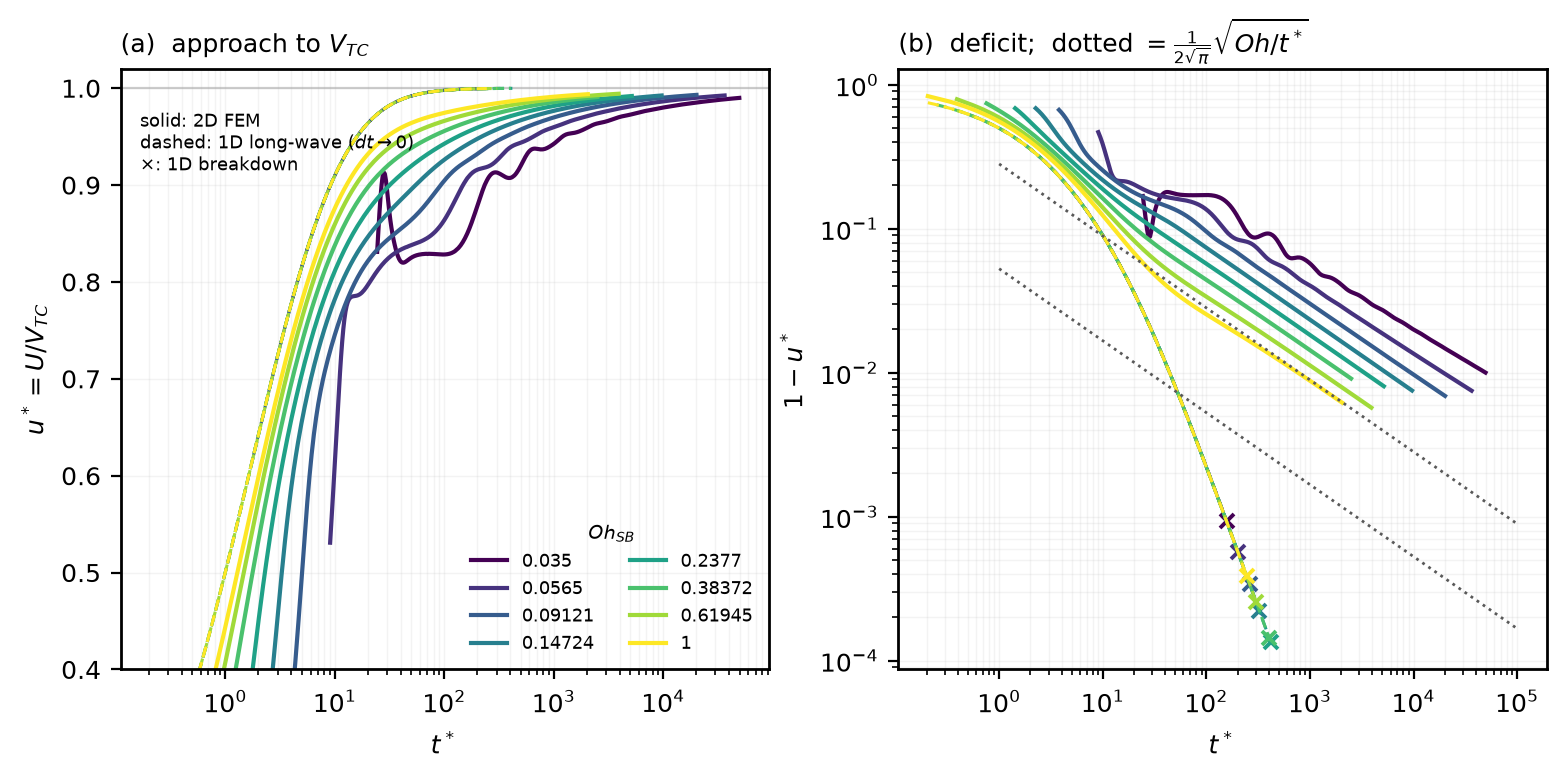
\includegraphics[width=\textwidth]{figures/fig5_1d_vs_2d.png}
  \caption{One-dimensional long-wave model against the two-dimensional
  finite-element solution. The reduced model is universal in $\tstar$. The
  two-dimensional solution is not.}
  \label{fig:onedtwod}
\end{figure}

Dropping inertia outright is not the viscous-limit reduction. An inertialess
balance forces a spatially uniform viscous stress, which no initially flat
sheet can satisfy. Inertia is what localises the disturbance near the edge.
What large $\mathrm{Oh}$ buys is that capillary stress leaves the bulk and
acts only through the edge condition.

Compared at matched $T$ against the converged reduced model, $\Ohp = 10$ tracks
it closely at first and then leaves it. Taking the slope gap exceeding $0.10$
as the operational boundary gives a window
\begin{equation}
  T_{\mathrm{dep}} \approx 0.84\,\Ohp^{0.48}
\end{equation}
over a factor $13$ in $\Ohp$. The window widens as $\sqrt{\Ohp}$, not as
$\Ohp$. That is not what the stated validity bound $T \ll \Ohp$ would lead one
to expect. Extrapolating the fit, a decade of long-wave validity
($T_{\mathrm{dep}} = 10$) requires $\Ohp \approx 170$, i.e.\ $\Ohsb \approx 85$.
That is a four-point extrapolation over one decade of $\mathrm{Oh}$ and should
be treated as an order of magnitude. The case that would test it is
$\Ohsb = 50$, which is not yet run.

\section{What is and is not established}
\label{sec:established}

\paragraph{Established.}
The co-moving formulation, and that the window (not the mesh) controls the
answer, converged for $L \ge 40$ at $\Ohsb = 1$.
$\ustar(\tstar=30) = 0.95026$ at $\Ohsb = 1$, converged in mesh, window and
timestep. A $0.41\%$ offset from the digitised Savva \& Bush value that is not
numerical. Temporal error below $10^{-4}$ across an eightfold change in output
cadence. The phenomenological sequence of figure~\ref{fig:phenomenology} across
a factor $29$ in $\mathrm{Oh}$.

The long-time limit. $v(t\to\infty) = \Vtc$ at every $\mathrm{Oh}$, approached
diffusively as
\begin{equation}
  1 - \ustar(\tstar)
  = \frac{1}{2\sqrt{\pi}}\,\sqrt{\Ohsb/\tstar}.
  \label{eq:deficit}
\end{equation}
Five cases spanning a factor $6.8$ in $\mathrm{Oh}$ sit within $1\%$ of the
constant $1/(2\sqrt{\pi}) = 0.28209$, namely $0.2837$, $0.2823$, $0.2816$,
$0.2813$, $0.2793$ at $\Ohsb = 0.14724$, $0.2377$, $0.38372$, $0.61945$,
$1.0$, with measured exponents $-0.4901$ to $-0.4998$ against the predicted
$-1/2$. Viscosity sets how slowly $\Vtc$ is reached, not what is reached.

The coefficient is established over that band and not beyond it. Outside
$0.14724 \le \Ohsb \le 1$ it departs in both directions. $+44\%$ at
$\Ohsb = 0.035$, and a factor of seven low at $\Ohsb = 5$, where the exponent
nonetheless returns to $-1/2$. The exponent is the robust feature. The
coefficient is not universal on the evidence available.

The inertial planar finite-element versus Basilisk comparison at
$\Ohsb < 0.1$. Terminal finite-element $\ustar$ is $0.994$--$0.996$. Basilisk
at $\Ohsb = 0.035$, taken to capillary time $t = 500$, is $\ustar \approx 0.977$.
The offset is the expected difference between a sharp free surface with no gas
and a diffuse two-phase interface. This is a statement about $\Vtc$, not about
the coefficient in~\eqref{eq:deficit} below $\Ohsb = 0.14724$.

The one-dimensional long-wave model is universal in $\tstar$ and the
two-dimensional solution is not, so the two cannot agree across $\mathrm{Oh}$
in principle.

\paragraph{Not established.}
What happens to the deficit coefficient at low $\mathrm{Oh}$. The three lowest
production cases sit outside~\eqref{eq:deficit}, and extending two of them
moved them further from $1/(2\sqrt{\pi})$, not toward it. At $\Ohsb = 0.035$
the deficit is not monotone, so no decaying power law can describe it. That
oscillation is rim dynamics at the inertial end of the range. Pierson
\textit{et al.}\ \cite{pierson2020} establish ringing about $\Vtc$ for an
axisymmetric filament at $\mathrm{Oh} \lesssim 0.1$. Nobody states it for the
planar sheet. Whether~\eqref{eq:deficit} is exact. Five cases agreeing to
within $1\%$ is suggestive of a closed form, not proof of one. How large
$\mathrm{Oh}$ must be for long-wave asymptotics in two dimensions. The
$\sqrt{\Ohp}$ window is a result. The inference that a decade of validity needs
$\Ohp \approx 170$ is an extrapolation. Anything at $\Ohsb > 1$, which is out
of scope for the production campaign. The single diagnostic case at
$\Ohsb = 5$ is reported only where \S\ref{sec:1d2d} needs it.

\section{Reproducing the figures}
\label{sec:repro}

Simulation output does not live in this repository. Runs write to the project
run root on the compute host. Custody is recorded in the project tracker. The
figure script takes paths to those run roots and skips any case whose data is
not mounted. From the repository root,
\begin{verbatim}
uv run python postProcess/make_docs_figures.py \
    --out docs/planar-campaign/figures
\end{verbatim}
The four campaign figures rebuild from that output.
Figure~\ref{fig:onedtwod} is produced by \texttt{postProcess/compare\_1d\_2d.py}.

\bibliographystyle{unsrt}
\bibliography{planar-campaign}

\end{document}
